\documentclass{sig-alternate-10pt}
%\documentclass[letterpaper,11pt]{article}
\usepackage{url}
%\usepackage{usenix,epsfig,endnotes}
%\usepackage{fullpage}
\setlength{\textheight}{9.5in}
%\setlength{\textwidth}{6.75in}
%\setlength{\oddsidemargin}{-.125in}
\usepackage{graphicx}
\usepackage{enumerate}
%\usepackage{subfigure}
%\usepackage{ifpdf}
%\usepackage{multicol}
%\usepackage{amsmath, amssymb, amsthm}
%\usepackage{rotating}
%\onehalfspacing
%\newcommand{\tbd}[1]{[{\bf{#1}}]}
\newcommand{\tbd}[1]{}
\newcommand{\ie}{{\it i.e.}}
\newcommand{\eg}{{\it e.g.}}
\newcommand{\etc}{{\it etc.}}
\newcommand{\eat}[1]{}
%\renewcommand\bibname{}

%\setlength\topmargin{0in}
%\usepackage{verbatim}
%\usepackage[compact]{titlesec}
%\usepackage[small]{caption}
\usepackage{times}

\title{Correspondence Checking for Computer Networks \\
\Large{CS 263 Project, Spring 2012 \vspace{-25pt}}}

\author{Colin Scott\thanks{In collaboration with Andi
Wundsam and Scott Shenker}\vspace{-15pt}}

\date{}
\begin{document}
    \maketitle
    \thispagestyle{empty}
\section{Background}

Many network invariant checks~\cite{HeaderSpace, Anteater} are specified in
terms of generally undesirable
states such as loops or blackholes.
In this project we discuss how to check more fine-grained,
application specific set of
invariants without requiring human involvement.
Our approach is to extract the network policies already reflected in the
network controller's data structures, and compare this to the actual state of
the physical network.
We refer to this technique as correspondence checking. Correspondence checking
builds on the virtual packet algebra
pioneered in headerspace analysis~\cite{HeaderSpace}.

\subsection{Model}

Computer networks can be represented as directed graphs:
\begin{align*}
G = (V, E)
\end{align*}

Forwarding elements are represented as internal vertices:
\begin{align*}
V_{fwd} = \{ v \in V |\text{ } degree(v) > 1 \}
\end{align*}

End-hosts are represented as edge vertices:
\begin{align*}
V_{host} = \{ v \in V |\text{ } degree(v) = 1 \}
\end{align*}

End-hosts send and receive packets. A packet's source and destination,
among other information, is encoded in the packet's header:
\begin{align*}
h \in \{0,1\}^L = H
\end{align*}
where $L$ is the maximum number of bits in
the header.

Upon receiving a packet, forwarding elements apply a transformation
function\footnote{We assume unicast forwarding for the purposes of this proposal}:
\begin{align*}
T: (H \times E) \rightarrow (H \times E_{\emptyset})
\end{align*}
Note that forwarding elements may rewrite fields of a packet header before passing it along.
Forwarding elements may also drop packets, in which case $T(.) = (.,\{\})$.

We use $`\Psi`$ to denote the collection of all transfer functions present in
the network at a particular point in time.

In this model, network traversal is simply a composition of transformation
functions. For example, if a header $h$ enters the network through edge
$e$, its state after $k$ hops will be:
\begin{align*}
\Phi^k(h,e) = \Psi(\Psi(\dots \Psi(h,e)\dots))
\end{align*}

Only end-hosts can insert new packets into the network\footnote{We ignore
control and diagnostic traffic for the purposes of this proposal}. The access links
of end-hosts are therefore the only entry and exit points for packets:
\begin{align*}
E_{access} = \{ (v_1,v_2) \in E |\text{ } v_1 \in V_{host} \vee v_2 \in V_{host} \}
\end{align*}

The externally visible behavior of the network is expressed as a relation between
packets originating from end-hosts and the packets' final locations:
\begin{align*}
\Omega: (H \times E_{access}) \rightarrow (H \times (E \cup
\{\emptyset, LOOP\})) \\
\Omega(h,e) = \Phi^{\infty}(h,e)
\end{align*}
We use the special value $LOOP$ to distinguish
a packet dropped by a network device from a packet entering an
infinite loop (both of which never leave the network).

\subsection{Software-defined Networks}

Software-defined Networking (SDN) is a paradigm for controlling network behavior.
SDN control software maintains a data-structure representing the global state of the
network. We refer to this data-structure as the `view`:
\begin{align*}
G^{view} = (V^{view},E^{view})
\end{align*}

Control programs running on top of the SDN controllers configure the network by
defining $\Psi^{view}$. The role of the platform is then to map $\Psi^{view}$ to
routing entries in the underlying forwarding elements of the
physical network. The physical network is also a graph:
\begin{align*}
G^{physical} = (V^{physical}, E^{physical}) 
\end{align*}

Note that the mapping between $G^{view}$ and $G^{physical}$ is not
necessarily one-to-one; the SDN control software may virtualize the view
such that a single member of $V_{fwd}^{view}$ maps to multiple members of
$V_{fwd}^{physical}$. A common pattern is to map a single forwarding element $v \in V_{fwd}^{view}$ to
an entire physical network $V_{fwd}^{physical}$. Figure \ref{fig:view_and_physical}
depicts an example. In the example, $V_{fwd}^{view} = \{ Switch \}$, and
$Switch$ maps onto:
\begin{align*}
\{ vswitch_1, vswitch_2, vswitch_3,  vswitch_4, \\
TOR_1 TOR_2, Gateway \} = V_{fwd}^{physical} 
\end{align*}

\begin{figure}[t]
\hspace{-10pt}
\begin{tabular}{c}
    $G^{view}$ \\
    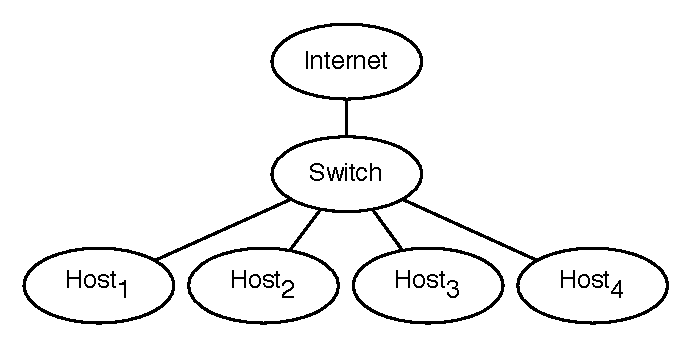
\includegraphics[width=3.25in]{../diagrams/necula_views/app_view.pdf}  \\
    $G^{physical}$ \\
    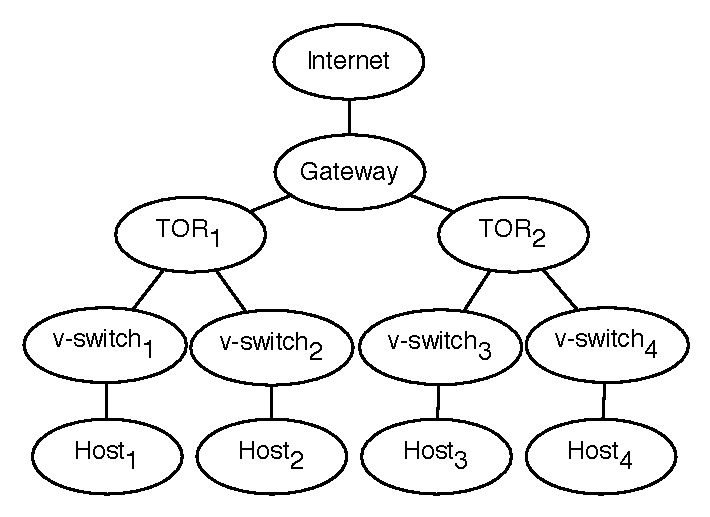
\includegraphics[width=3.25in]{../diagrams/necula_views/physical_view.pdf}
\end{tabular}
\caption[]{\label{fig:view_and_physical} Example correspondence between
$G^{view}$ and $G^{physical}$. In the view a single switch connects 
four hosts and the rest of the Internet (modeled as a single vertex).
This single switch is mapped onto four v-switches, two top-of-rack switches 
and one gateway router in the physical network.}
\end{figure}

As we will see later on, it is important to note that there is still a one-to-one correspondence
between $V_{host}^{view}$ and $V_{host}^{physical}$, as well as between
$E_{access}^{view}$ and $E_{access}^{physical}$.

\section{Problem Statement}

It should always be the case that 
$\Omega^{view} \sim \Omega^{physical}$. Formally:
\begin{align*}
\forall_{h} \forall_{e \in E_{access}^{view}} \Omega^{view}(h,e) =
\Omega^{physical}(encap(h),\hat{e}) 
\end{align*}
where $encap$ is a function from packets in $G^{view}$ to packets in
$G^{physical}$, and $e \sim \hat{e} \in E_{access}^{physical}$.

In practice however, there are often miscorrespondence between the two. Some
of these miscorrespondence are innocuous; networks are distributed systems,
and there are inevitable delays between updates in $G^{view}$ and the
corresponding changes in $G^{physical}$. Other miscorrespondence are
due to critical bugs in SDN control software. In general, controller software
is a
highly complex piece of software; it must deal with hardware-faults,
communication delays, and complex mapping functions  between $G^{view}$ and
$G^{physical}$. Moreover, production networks may contain  $10's$ of thousands of
forwarding devices. In such an environment, the control program must be
replicated across multiple servers to handle the load and ensure
fault-tolerance. The SDN control software must ensure that $G^{view}$ remains consistent
between all replicas despite server failures, communication delays, and
message re-orderings.

\section{Algorithm}

Correspondence checking verifies
correspondence between $\Omega^{view}$ and $\Omega^{physical}$.
It works as follows:
\begin{enumerate}[i.]
\item Take a distributed snapshot of $G^{physical}$ \cite{distributedsnapshots}
\item Translate the routing tables of $V_{fwd}^{physical}$ into transformation
functions $\Psi^{physical}$
\item Feed a symbolic packet $h_s$ through each access link $e \in E_{access}$
\item Track the progress of $h_s$ through the network, thereby computing
$\Omega^{view}$. If a packet
enters a loop before exiting the network, we mark the value as
$LOOP$. Otherwise,
the leaves of the propagation graph define the final outcomes of the input
packets injected at that access link.
\item Do the same for $G^{view}$
\item Because network policies are defined by
configuring the logical view, any mismatch between $\Omega^{view}$ and $\Omega^{physical}$
represents an instance of a correctness violation. Note that mismatches are
unambiguous; that is, two slightly different correctness violation from
different runs of the system are always distinguishable.
We therefore seek to identify counterexamples:
\begin{align*}
 \{ (h,e) |\text{ } h \in H, e \in E^{view}_{access} \sim
 E^{physical}_{access}, \\
 \Omega^{view}(h,e) \neq  \Omega^{physical}(encap(h),e) \}
\end{align*}
\end{enumerate}


\section{Limitations}

Note the price of correspondence checking's generality is that it represents
a somewhat weak notion of
correctness. Correspondence checking only captures external behavior and
loops; it does not capture internal behavior such as load-balancing
over links. It also assumes that the policies as expressed by the
configuration of the logical view are correct. Finally, correspondence
checking can not verify
time-dependent policies such as ``No link should be congested more than 1\% of
the time''.

\scriptsize
\bibliographystyle{abbrv}
\bibliography{bib}

%\input{appendix}
\end{document}
